%% Bookheader, Nov 8, 2020; July 18, 2022

\documentclass[11pt]{../Support/ourbook}
%% or for landscape, comment out line above and use this one:
%%\documentclass[landscape,11pt]{ourbook}

%% This will keep space from stretching around display math:

\makeatletter
\renewcommand\normalsize{%
   \@setfontsize\normalsize\@xipt{13.6}%
   \abovedisplayskip 11\p@  \@minus6\p@
   \abovedisplayshortskip \z@ 
   \belowdisplayshortskip 6.5\p@ \@minus3\p@
   \belowdisplayskip \abovedisplayskip
   \let\@listi\@listI}
\makeatother
\normalsize


\begin{document}

\tableofcontents
\graphicspath{{../../Chapters/emwaves/en_US}}
\chapter{Introduction to the Kontinua Sequence}

This book will start you on the long and difficult trek to becoming a modern
problem solver. Along the path, you will learn how to use the tools of
math, computers, and science.

Why should you bother? There are big problems in this world that will
require expert problem solvers. Those people will make the world a
better place while enjoying interesting and lucrative careers. We are
talking about engineers, scientists, doctors, computer programmers,
architects, actuaries, and mathematicians. Right now, those occupations represent
about 6\% of all the jobs in the United States. Soon,
that number is expected to rise above 10\%.  On average, people in
that 10\% of the population are expected to have salaries twice that
of their non-technical counterparts.\index{career}

Solving problems is difficult. At some point on this journey, you will
see people who are better at solving problems than you are. You, like
every other person who has gone on this journey, will think ``I have
worked so hard on this, but that person is better at it than
I am. I should quit.'' Don't.\index{quitting}

First, solving problems is like a muscle. The more you do, the better
you get at it.  It is OK to say ``I am not good at this yet.'' That
just means you need more practice.

Second, you don't need to be the best in the world. 10 million people
your age can be better at solving problems than you, \textit{and you
  can still be in the top 10\% of the world}. If you complete this
journey, there will be problems for you to solve and a job where your
problem-solving skills will be appreciated.

\emph{Where do we start?}

The famous physicist Richard Feynman once asked this question: ``If,
in some cataclysm, all of scientific knowledge were to be destroyed,
and only one sentence was passed on to the next generation of
creatures, what statement would contain the most information in the
fewest words?''

His answer was ``All things are made of atoms—little particles that move around in
perpetual motion, attracting each other when they are a little
distance apart, but repelling upon being squeezed into one another.''

\emph{That} seems like a good place to start.

\graphicspath{{../../Chapters/camera/en_US}}
\chapter{How Cameras Work}

Let's say it is a sunny day and you are standing in a field a few meters
from a cow. You use the camera on your phone to take a picture of the
cow. How does that whole process work?

\section{The Light That Shines On the Cow}

The sun is a sphere of hot gas. About 70\% of the gas is
hydrogen. About 28\% is helium. There's also a little carbon, nitrogen,
and oxygen.

Gradually, the sun is converting hydrogen into helium through a
process known as ``nuclear fusion''. (We will talk more about nuclear
fusion in a later chapter.) A lot of heat is created in this
process. The heat makes the gases glow.

How does heat make things glow? The heat pushes the electrons into
higher orbitals.  When they back down to a lower orbital, they
release a photon of energy, which travels away from the atom as an
electromagnetic wave.

Heat isn't the only way to push the electrons into a higher
orbital. For example, a fluorescent lightbulb is filled with gas.
When we pass electricity through the gas, its electrons are moved to a
higher orbital.  When they fall, light is created.

What is the frequency of the wave that the photon travels on?
Depending on what orbital it falls from and how far it falls, the
photon created has different amounts of energy. The amount of energy
determines the frequency of the electromagnetic wave.

\begin{mdframed}[style=important, frametitle={Formula for enegy of a photon}]

If you want to know the amount of energy $E$ in a photon, here is the formula:

$$E = \frac{h c}{\lambda}$$

where $c$ is the speed of light, $\lambda$ is the wavelength of the
electromagnetic wave, and $h$ Planck's constant: $6.63 \times 10^{-34} m^2 kg/s$

For example, a red laser light has a wavelength of about 630 nm. So the energy in each photon is:

$$\frac{(300 \times 10^6) (6.63 \times 10^{-34})}{630 \times 10^{-9}} = 3.1 \times 10^{-19} \text{ joules}$$

\end{mdframed}

In the sun, there are several kinds of molecules and each has a few
different orbitals that the electrons can live in.  Thus, the light
coming from the sun is made up of electromagnetic waves of many
different frequencies.

We can see some of these frequencies as different colors, but some are
invisible to humans, for example ultraviolet and infrared.

\section{Light Hits the Cow}


When these photons from the sun hit the cow, the hide and hairs of the
cow will absorb some of the photons. These photons will become heat
and make the cow feel warm.  Some of the photons will not be absorbed
-- they will leave the cow.  When you say ``I see the cow,'' what you are
really saying is ``I see some photons that were not absorbed by the cow.''

Different materials absorb different amounts of each wavelength. A
plant, for example, absorbs a large percentage of all blue and red
photons that hit it, but it absorbs only a small percentage of the
green photons that hit it.  Thus we say ``That plant is green.''

White things absorb very small percentages of photons of any visible
wavelength.  Black things absorb very \emph{large} percentages of
photons of any visible wavelength.

Before we go on, let's review: The sun creates photons that travel as
electromagnetic waves of assorted wavelengths to the cow.  Many of
those photons are absorbed, but some are not.  Some of those photons
that are not absorbed go into the lens of our camera.

\section{Pinhole camera}

The simplest cameras have no lenses. They are just a box.  The box has
a tiny hole that allows photons to enter.  The side of the box
opposite the hole is flat and covered with film or some other
photo-sensitive material.

The photons entering the box continue in the same direction they were
going when they passed through the hole.  Thus, the photons that
entered from high, hit the back wall low.  The photons that came from
the left, hit the back wall on the right. Thus the image is projected
onto the back wall rotated 180 degrees: What was up is down, what was
on the left is on the right.

\includegraphics[width=1\textwidth]{pinholeCamera.png}


\begin{Exercise}[title={Height of the image}, label=image_height]

FIXME: cow swap

Let's say that that the pinhole is exactly the same height as the
shoulder of the cow and that the shoulder is directly above one hoof.
Than the pinhole, the shoulder, and the hoof form a right triangle.

Now, let's say that the camera is being held perpendicular to the
ground.  Now, the pinhole, the image of the shoulder, and the image of
the hoof on the back wall of the camera also form a right triangle.

These two triangles are similar.

The shoulder is 2 meters from the hoof.  The cow is standing 3 meters
from the camera.  The distance from the pinhole to the back wall of
the camera is 3 cm.  How tall is the image of the cow on the back wall
of the camera?

\end{Exercise}
\begin{Answer}[ref=image_height]

The two triangles are similar, one is 2 m and 3m.  The other is $x$ cm and 3 cm.

The image of the cow is 2 cm tall.

\end{Answer}

\section{Lenses}

Quick review: A photon leaves the sun in some random direction. It
travels 150 million km from the sun and hits a cow.  It is not
absorbed by the cow, and heads off in a new direction.  It passes
through the pinhole and hits the back wall of the camera.  That seems
incredibly improbable, right?

It actually is kind of improbable, especially if there isn't a lot of
light -- like you are taking the picture at dusk.  To increase the
odds, we added a \newterm{lens} to the camera.

If you focus a lens on a wall, and then you draw a dot on the
wall. The lens is designed such that all the photons from the dot that
hit the lens get redirected to the same spot on the back wall of the
camera -- regardless of which path it took to get to the lens.

\includegraphics[width=1\textwidth]{pinholePoints.png}



Note that the image still gets flipped.  There is a \newterm{ focal
point } that all the photons pass through.

\includegraphics[width=1\textwidth]{lensPoints.png}

The distance from the lens to its focal point is called the lens's
\newterm{focal length}. Telephoto lenses, that let you take big
pictures of things that are far away, have long focal lengths.
Wide-angle lenses have short focal lengths.

\section{Sensors}

The camera on your phone has a sensor on the back wall of the
camera. The sensor is broken up into tiny rectangular regions called
pixels.  When you say a sensor is 6000 by 4000 pixels, we are saying
the sensor is a grid of 24,000,000 pixels: 6000 pixels wide and
4000 pixels tall.

Each pixel has three types of cavities that take in photos. One of the
cavities measures the amount of short wavelength light, like blues and
violets. One of the cavities measures the long wavelength light, like
reds and oranges. One of the cavities measures the intensity of
wavelengths in the middle, like greens.

Thus, if your camera has a resolution of $6000 \times 4000$, the image
is 72,000,000 numbers: Every one of the 24,000,000 pixels yeilds three
numbers: intensity of long wavelength, mid wavelength, and long
wavelength light. We call these numbers ``RGB'' for Red, Green, and
Blue.




\graphicspath{{../../Chapters/eye/en_US}}
\chapter{How Eyes Work}

Dr. Craig Blackwell has made a great video on the mechanics of the
eye. You should watch it: \url{https://youtu.be/Z8asc2SfFHM}

Mechanically, your eye works a lot like a camera.  The eye is a sphere
with two lenses on the front: The outer lens is called the \newterm{cornea}, the
second lens is just called ``the lens.''

Between the two lenses is an aperature that opens wide when there is
very little light, and closes very small when there is bright light.
The opening is called the \newterm{pupil} and the tissue that forms
the pupil is called the \newterm{iris}.  When people talk of the color
of your eyes, they are talking about the color of your iris. The
blackness at the center of your iris is your pupil.

There are two types of photoreceptor cells in your retina: rods and
cones. The rods are more sensitive; in very dark conditions, most of
our vision is provided by the rods. The cones are used when there is
plenty of light, and they let us see colors.

The white part around the outside of theeyeball? That is called the
\newterm{sclera}.

\includegraphics[width=0.8\textwidth]{eye.png}

The walls of the eye are lined inside with the \newterm{retina}, which has
 sensors that pick up the light and send impulses down the optic
nerve to your brain.

Just like a camera, the images are flipped when they get projected on
the back of the eye.

\section{Eye problems}

Now that you know the mechanics of the eye, let's enumerate a few
things that commonly go wrong with the eye.

\subsection{Glaucoma}

The space between your cornea and lens is filled with a fluid called
\newterm{aqueous humour}. To feed the cells of the cornea and lens,
the aqueous humour carries oxygen and nutrients like blood would, but
it is transparent so you can see. Aqueus humour is constantly being
pumped into and out of that chamber.  If aqueus humour has trouble
exiting, the pressure builds up and can damage the eye. This is known
as \newterm{glaucoma}.

\subsection{Cataracts}

The lens should be clear. As a person ages (and it can be accelerated
by diabetes, too much exposure to sunlight, smoking, obesity, and high
blood pressure), the proteins in the lens break down and clump
together, becoming opaque. From the outside, the eye will look
cloudy. This is called a \newterm{cataract}, and it makes it difficult
for the person to see.

The problem can be corrected: The person's cloudy lens is removed and
replaced with a clear, manufactured lens.

\subsection{Nearsightedness, farsightedness, and astigmatism}

If you are in a dark room and a tiny LED is turned on, the photons
from that LED can pass through your cornea in many different places.
If your eye is focusing on that light correctly, all the photons
should meet up at the same place on the retina.

FIXME: Diagram here

If the lenses are bending the light too much, the photons meet up before they hit the
retina and get smeared a bit across the retina. To the person, the LED
would appear blurry. The eye is said to be \newterm{nearsighted} or
\newterm{myopic}.

If the lenses are not bending them enough, the photons would meet up
behind the retina.  Once again, they get smeared a bit across the
retina and the LED looks blurry to the person. The eye is said to be
\newterm{farsighted} or \newterm{hyperoptic}.

Your lenses are supposed to bend the photons the same amount
vertically and horizontally. If one dimension is focused, but the
other is myopic or hyperoptic, the eye is said to have \newterm{astigmatism}.

Myopia, hyperoptia, and astigmatism can be corrected with glasses or contact
lenses. Doctors can also do surgical corrections, usually by changing
the shape of the cornea.

\section{Seeing colors}

TED-Ed has made a good video on how we see color. Watch it here: \url{https://youtu.be/l8_fZPHasdo}

When a rainbow forms, you are seeing different wavelengths separating from each other. In the rainbow:
\begin{itemize}
\item Red is about 650 nm.
\item Orange is about 600 nm.
\item Yellow is about 580 nm.
\item Green is about 550 nm.
\item Cyan is about 500 nm.
\item Blue is about 450 nm.
\item Violet is about 400 nm.
\end{itemize}

If you shine a light with a wavelength of 580 nm on a white piece of
paper, you will see yellow.

However, if you shine two lights with wavelengths of 650 nm (red) and
550 nm (green), you will also see yellow.

Why? Our ears can hear two different frequencies at the same time.
Why can't our eyes see two colors in the same place?

As mentioned above, the cone photoreceptors in our eyes let us see
colors. There are three kinds of cones:
\begin{itemize}
  \item Blue: Cones that are most sensitive to frequencies near 450nm.
  \item Green: Cones that are most sensitive to frequencies near 550nm.
  \item Red: Cones that let us see the frequencies up to about 700nm.
\end{itemize}

When a wavelength of 580 nm hits your retina, it excites the red
and green receptors, and your brain interprets that mix as yellow.

Similarly, when light that contains both 650 nm and 550 nm waves hits
your retina, it excites the red and green receptors, and your brain
interprets that mix as yellow.

You can't tell the difference!

Now we know why the sensors on the camera are RGB. The camera is
recording the scene as closely as necessary to fool your eye.

A TV or a color computer monitor only has three colors of pixels: red,
green, and blue.  By controlling the mix of them, it creates the
sensation of thousands of colors to your eye.

\section{Pigments}

A color printer works in the opposite manner: Instead of radiating
colors, it puts pigments on the paper that absorb certain freqencies.
A pigment that absorbs only frequencies near 650 nm (red) will appear
to your eye as cyan. This makes sense because the sensation of cyan is
created when your blue and green receptors are activated.

Thus, pigment colors come in:
\begin{itemize}
\item Cyan: absorbs frequencies around red
\item Magenta: absorbs freqencies around green
\item Yellow: absorbs frequencies around blue
\end{itemize}

If you buy ink for a color printer, you know there is typically a
fourth ink: black. If you put cyan, magenta, and yellow pigments on
paper, the mix won't absorb all the visible spectrum in a consistent
manner, and our eyes are pretty sensitive to that, so we would see
brown. So we add black ink to get pretty grays and blacks.

We call this approach to color CMYK (as opposed to RGB). If an artist
is creating an image to be viewed on a screen, they will typically
make an RGB image.  If they are creating an image to be printed using
pigments, they typically create a CMYK image. (Most of us don't care
so much -- we just let the computer do conversions between the two
color spaces for us.)


\graphicspath{{../../Chapters/reflection/en_US}}
\chapter{Reflection}

Light reflection is the phenomenon where light waves bounce off a surface upon encountering it. It obeys the law of reflection, which states that the angle of incidence, denoted as $\theta_i$, is equal to the angle of reflection, denoted as $\theta_r$. This law can be mathematically expressed as:

$$\theta_i = \theta_r$$
 
where $\theta_i$ is the angle between the incident light ray and the normal to the surface, and $\theta_r$ is the angle between the reflected light ray and the normal.

To understand the math behind light reflection, we can consider a plane mirror as an example. When a light ray hits a plane mirror, it is reflected back in a way that the incident angle is equal to the reflected angle with respect to the mirror's surface.

Let's assume the incident light ray is represented by a vector $\mathbf{i}$ and the normal to the mirror's surface is represented by a vector $\mathbf{n}$. The angle of incidence, $\theta_i$, can be calculated using the dot product between the incident ray and the normal:

$$\cos(\theta_i) = \frac{{\mathbf{i} \cdot \mathbf{n}}}{{\|\mathbf{i}\| \|\mathbf{n}\|}}$$
​	
 
where $\cdot$ denotes the dot product and $|\mathbf{i}|$ and $|\mathbf{n}|$ represent the magnitudes of the incident ray and the normal vector, respectively.

Since the law of reflection states that $\theta_i = \theta_r$, we can calculate the angle of reflection, $\theta_r$, using the inverse cosine function:

$$\theta_r = \cos^{-1}\left(\frac{{\mathbf{i} \cdot \mathbf{n}}}{{\|\mathbf{i}\| \|\mathbf{n}\|}}\right)$$

Once we have the angle of reflection, we can obtain the reflected ray by rotating the incident ray by an angle of $2\theta_r$ with respect to the mirror's surface. This can be done using rotation matrices or trigonometric functions, depending on the coordinate system being used.

In summary, light reflection follows the law of reflection, where the incident angle is equal to the reflected angle. By calculating the dot product between the incident ray and the surface's normal, we can determine the angles of incidence and reflection. Then, by rotating the incident ray, we can find the direction of the reflected ray.
\graphicspath{{../../Chapters/refraction/en_US}}
\chapter{Refraction}


Refraction of light is the phenomenon where light changes its direction when it passes from one medium to another. The change in direction is due to a change in the speed of light as it moves from one medium to another. 

This phenomenon is explained by Snell's law, which states:

\begin{equation}
n_1 \cdot \sin(\theta_1) = n_2 \cdot \sin(\theta_2)
\end{equation}

where:
\begin{itemize}
\item $n_1$ and $n_2$ are the indices of refraction for the first and second media, respectively. The index of refraction is the ratio of the speed of light in a vacuum to the speed of light in the medium. It is a dimensionless quantity.
\item $\theta_1$ and $\theta_2$ are the angles of incidence and refraction, respectively. These angles are measured from the normal (perpendicular line) to the surface at the point where light hits the boundary.
\end{itemize}

\includegraphics[width=.75\textwidth]{refraction.png}

The angle of incidence ($\theta_1$) is the angle between the incident ray and the normal to the interface at the point of incidence. Similarly, the angle of refraction ($\theta_2$) is the angle between the refracted ray and the normal.

When light travels from a medium with a lower refractive index to a medium with a higher refractive index, it bends towards the normal. Conversely, when light travels from a medium with a higher refractive index to one with a lower refractive index, it bends away from the normal.


\graphicspath{{../../Chapters/lens/en_US}}
\chapter{Lenses}

Lenses are optical devices with perfect or approximate axial symmetry
that transmit and refract light, converging or diverging the
beam. There are two main types of lenses, distinguished by their shape
and the way they refract light:\index{lenses}

\begin{itemize}
    \item \textbf{Converging (or Convex) Lenses:} These are thicker at
      the center than at the edges. When parallel light rays enter a
      convex lens, they converge to a point called the focal
      point. Examples of converging lenses include magnifying glasses
      and camera lenses.

      \includegraphics[width=0.5\textwidth]{convex.png}

    \item \textbf{Diverging (or Concave) Lenses:} These are thinner at
      the center than at the edges. When parallel light rays enter a
      concave lens, they diverge or spread out. These lenses are often
      used in glasses to correct nearsightedness.
      
      \includegraphics[width=0.5\textwidth]{concave.png}

\end{itemize}

\section{Focal Length}

The focal length of a lens is the distance between the center of the
lens and the focal point. It is determined by the lens shape and the
refractive index of the lens material. For a converging lens, the
focal length is positive, and for a diverging lens, the focal length
is negative.\index{focal length}

\section{Refractive Index}

The refractive index of a material is a measure of how much the speed
of light is reduced inside the material. The refractive index $n$ of a
material is given by the ratio of the speed of light in a vacuum $c$
to the speed of light $v$ in the material:\index{refractive index}

\[
n = \frac{c}{v}
\]

The refractive index affects how much a light ray changes direction,
or refracts, when entering the material at an angle. A higher
refractive index indicates that light travels slower in that medium
and the light ray will bend more towards the normal.

Lenses work by refracting light at their two surfaces. By choosing the
right lens shape and material, lenses can be designed to bring light
to a focus, spread it out, or perform more complex transformations.

\graphicspath{{../../Chapters/py_images/en_US}}
\chapter{Introduction to the Kontinua Sequence}

This book will start you on the long and difficult trek to becoming a modern
problem solver. Along the path, you will learn how to use the tools of
math, computers, and science.

Why should you bother? There are big problems in this world that will
require expert problem solvers. Those people will make the world a
better place while enjoying interesting and lucrative careers. We are
talking about engineers, scientists, doctors, computer programmers,
architects, actuaries, and mathematicians. Right now, those occupations represent
about 6\% of all the jobs in the United States. Soon,
that number is expected to rise above 10\%.  On average, people in
that 10\% of the population are expected to have salaries twice that
of their non-technical counterparts.\index{career}

Solving problems is difficult. At some point on this journey, you will
see people who are better at solving problems than you are. You, like
every other person who has gone on this journey, will think ``I have
worked so hard on this, but that person is better at it than
I am. I should quit.'' Don't.\index{quitting}

First, solving problems is like a muscle. The more you do, the better
you get at it.  It is OK to say ``I am not good at this yet.'' That
just means you need more practice.

Second, you don't need to be the best in the world. 10 million people
your age can be better at solving problems than you, \textit{and you
  can still be in the top 10\% of the world}. If you complete this
journey, there will be problems for you to solve and a job where your
problem-solving skills will be appreciated.

\emph{Where do we start?}

The famous physicist Richard Feynman once asked this question: ``If,
in some cataclysm, all of scientific knowledge were to be destroyed,
and only one sentence was passed on to the next generation of
creatures, what statement would contain the most information in the
fewest words?''

His answer was ``All things are made of atoms—little particles that move around in
perpetual motion, attracting each other when they are a little
distance apart, but repelling upon being squeezed into one another.''

\emph{That} seems like a good place to start.

%%%%%%%%%%%%%%%%%%%%%%%%%%%%%%%%%
%% Bookfooter.tex by Aaron Hillegass
%% Nov 8, 2020

\appendix

\chapter{Answers to Exercises}
\shipoutAnswer

\bibliography{references}

\printindex

\end{document}